\documentclass[a4paper,11pt]{article}
\author{ 杨旭鹏  \  PB17000234}
\date{2019年秋季}
\title{计算物理A 第一题}

\usepackage{ctex}
\usepackage{amsmath}
\usepackage{amsfonts}
\usepackage{graphicx}
\usepackage{lastpage}
\usepackage{hyperref}
\usepackage{listings}
\RequirePackage{xcolor}
\usepackage{appendix}
\makeatletter\def\@captype{table}\makeatother
\definecolor{dkgreen}{rgb}{0,0.6,0}
\definecolor{gray}{rgb}{0.5,0.5,0.5}
\definecolor{mauve}{rgb}{0.58,0,0.82}


\definecolor{dkgreen}{rgb}{0,0.6,0}
\definecolor{gray}{rgb}{0.5,0.5,0.5}
\definecolor{mauve}{rgb}{0.58,0,0.82}

\lstset{
  frame=tb,
  aboveskip=3mm,
  belowskip=3mm,
  showstringspaces=false,
  columns=flexible,
  framerule=1pt,
  rulecolor=\color{gray!35},
  backgroundcolor=\color{gray!5},
  basicstyle={\small\ttfamily},
  numbers=left,
  numberstyle=\tiny\color{gray},
  keywordstyle=\color{blue},
  commentstyle=\color{dkgreen},
  stringstyle=\color{mauve},
  breaklines=true,
  breakatwhitespace=true,
  tabsize=3,            
  }



\begin{document}
\maketitle

\section{题目描述}
用Schrage方法编写随机数子程序,用连续两个随机数作为点的坐标值绘出若干点的平面分布图。再用$<x^{k}>$测试均匀性(取不同量级的$N$值,讨论偏差与$N$的关系)、$C(l)$ 测试其2维独立性 (总点数$N>10^{7}$)。

\section{算法及程序思路}
\subsection{算法}
利用均匀随机数产生器中最简单的线性同余法实现随机数的产生,其方法为:

\begin{equation}
\begin{aligned}
	I_{n+1} &= (aI_{n} + b) \ mod \ m \\
	x_{n} &= I_{n}/m
\end{aligned}
\label{linear}	
\end{equation}

其中整数$I_{i} \in [0,m-1]$,$a,b,m$为算法中的可调参数,其选取直接影响产生器的质量。本程序使用的为具有“最低标准”的16807产生器,即:

\begin{equation}
\left\{
\begin{array}{l}
	a = 7^{5} = 16807 \\
	b = 0 \\
	m = 2^{31}-1 = 2147483647
\end{array}
\right.
\end{equation}

由于直接利用\ref{linear}编写程序时计算$(aI_{n} \ mod \ m )$时很容易造成数据溢出,故采取作业要求的Schrage方法进行具体编程的实现:

\begin{equation}
	aI_{n} \ mod \ m = \left\{
	\begin{array}{l}
		a(I_{n}\ mod \ q) - r[I_{n}/q],\ \ \ \ \ \ \ \ if \geq 0 \\
		a(I_{n}\ mod \ q) - r[I_{n}/q] + m,\ \ otherwise	
			\end{array}
	\right.
\end{equation}

其中$m=aq+r$,即$q=m/a=127773$,$r=m \ mod \ a=2836$。即可利用此方法产生伪随机数序列。

\subsection{程序思路}
首先我们需要产生一个随机数种子,最简单的方法便是人工赋值。也可读取相应的时间做种子例如在C语言下,可读取时间放入srand()函数中,并用rand()函数产生种子;在Linux系统下可读取"/dev/random"文件来得到相对“真”的随机数作为种子等等。\footnote{对于Linux下的“/dev/random”文件在Linux manual page 上有如下解释:The random number generator gathers environmental noise from device
       drivers and other sources into an entropy pool.  The generator also
       keeps an estimate of the number of bits of noise in the entropy pool.
       From this entropy pool, random numbers are created.可以看出此种方法产生的随机数并非来自于算法,而来自于热噪声。}在此程序中,我们采用最为简单的人工赋值法,这样做的好处是数据具有可重复性,方便后期的Debug。\footnote{在原版程序中,采取的是读取“/dev/random”文件方案}

产生随机种子后,利用递推公式:
\begin{equation}
	I_{n+1} = aI_{n}  \ mod \ m = \left\{
	\begin{array}{l}
	a(I_{n}\ mod \ q) - r[I_{n}/q],\ \ \ \ \ \ \ \ if \geq 0 \\
		a(I_{n}\ mod \ q) - r[I_{n}/q] + m,\ \ otherwise	 \\
		a= 7^{5} =16807 \\
		q=m/a=127773\\
		r=m \ mod \ a=2836
	\end{array} 
	\right.
\end{equation}

计算随机数列。

得到随机数列后,将奇数项放入一个数组作为坐标$x$的值,偶数项放入另一个数组作为坐标$y$的值,然后将两个数组的数据输出到.dat文件中,以便后期画图处理。\footnote{本程序利用python脚本,使用matplotlib绘制图样}数据的$<x^{k}>$测试以及$C(l)$ 测试,也相应的进行,详情请见代码。

\section{程序使用方法}
在运行程序后,会看到请求输入所需总随机点数的提示,按照提示在后面输入所需要的总随机点数,摁回车继续。然后经过计算给出所有随机数点的线性相关系数$C(l)$计算结果并输出随机数.dat文件至当前文件夹。然后按照程序提示,输入所需计算的$<x^{k}>$中$k$的最大值,按回车继续程序,会自动在屏幕上显示从总点数次方量级的10\% 到 100\% ,从$k=1$到您输入的最大值的$<x^{k}>$和$<y^{k}>$的计算值及均匀分布的理论值。程序输出完这些后会自动退出。
\begin{figure}[!htbp]        
\center{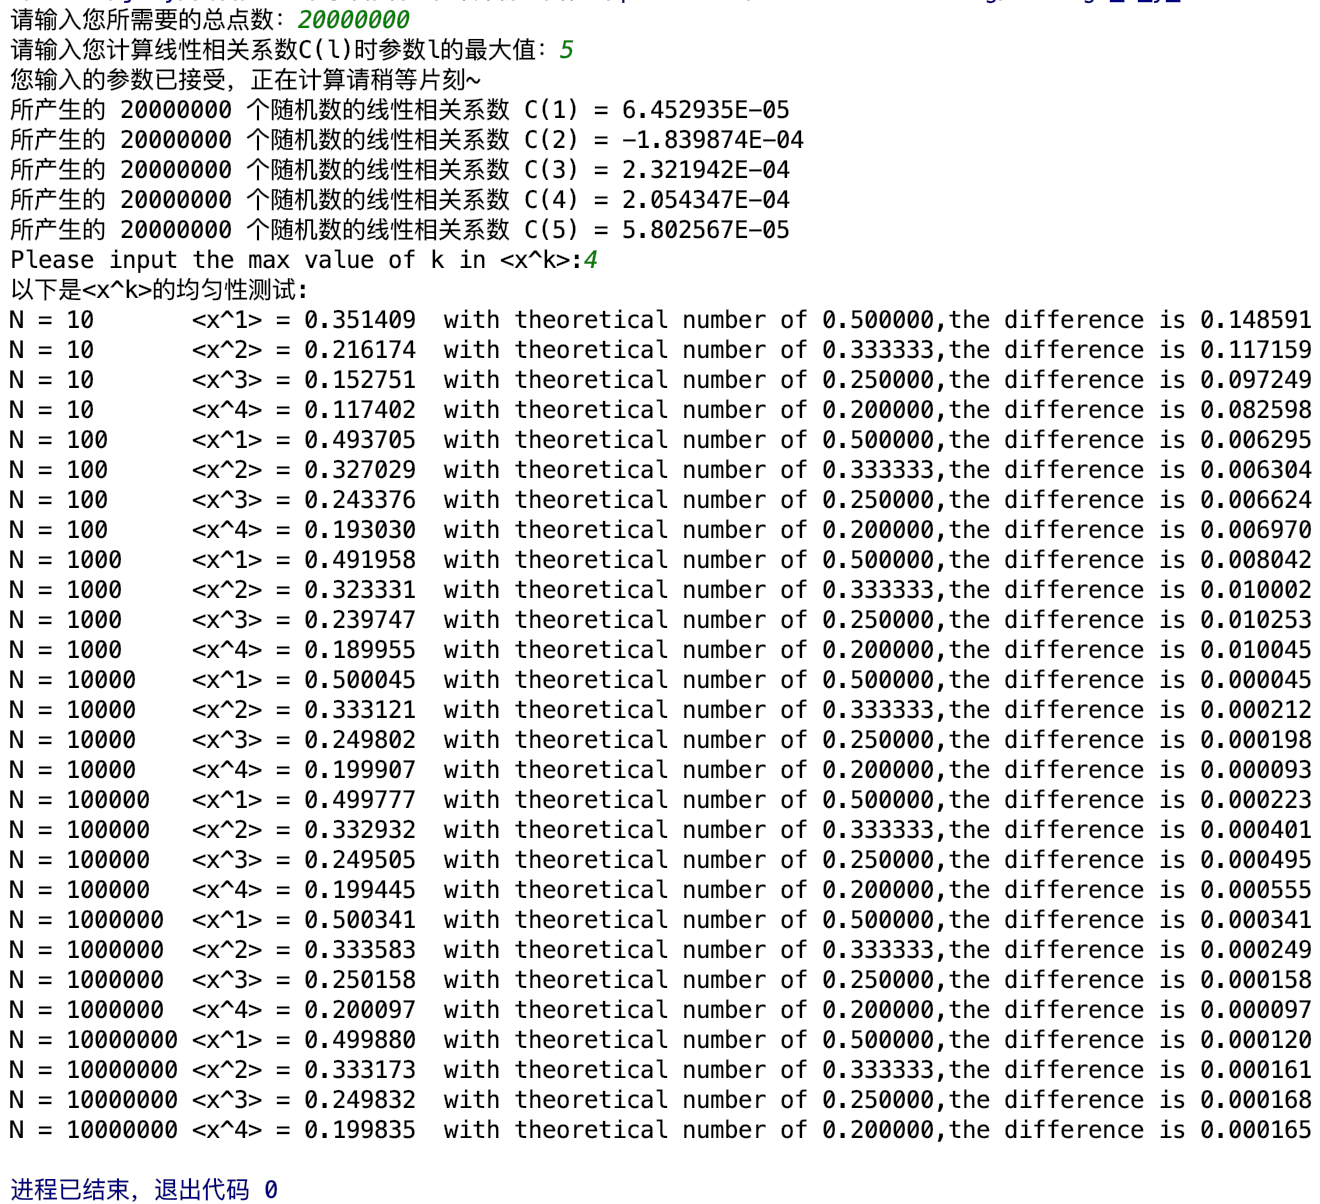
\includegraphics[width=11cm]  {example.png}}        
\caption{\label{1} 一个典型程序的运行过程示例}      
\end{figure}


\section{程序结果与分析}
当设定初始种子值为“1”时,利用python脚本我们得到如下可视化后的数据:

\begin{figure}[!htbp]        
\center{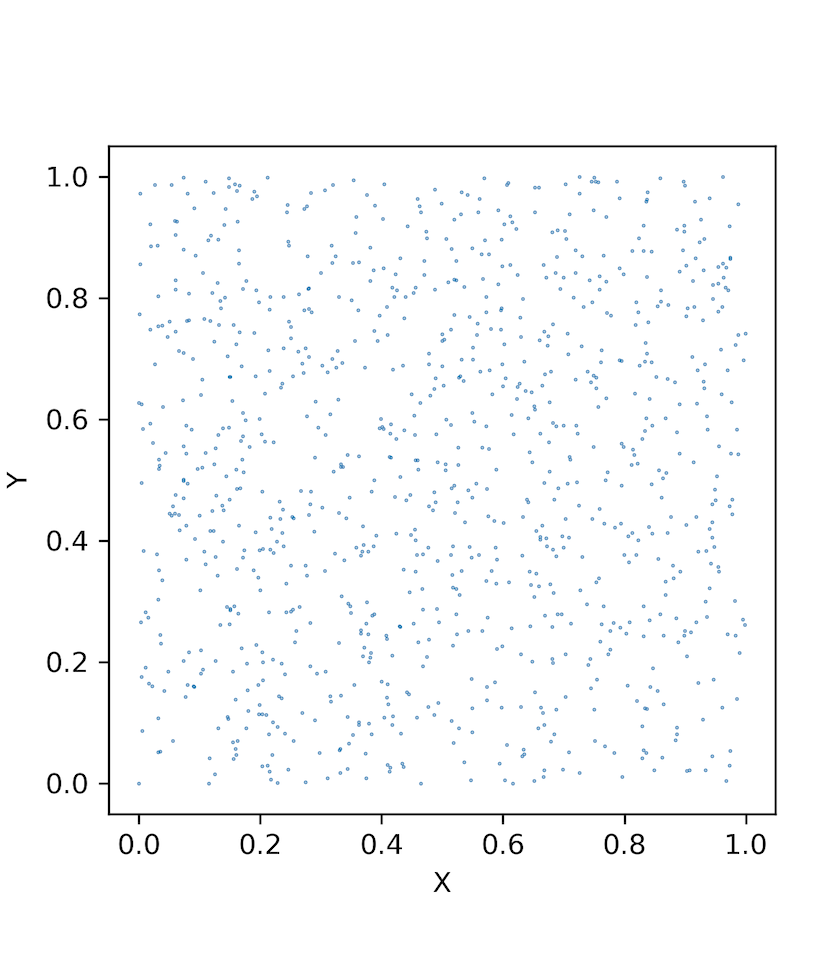
\includegraphics[width=14cm]  {103.png}}        
\caption{\label{1} 由种子“1”生成的$1 \times 10^{3}$个均匀分布随机点}      
\end{figure}


\begin{figure}[!htbp]        
\center{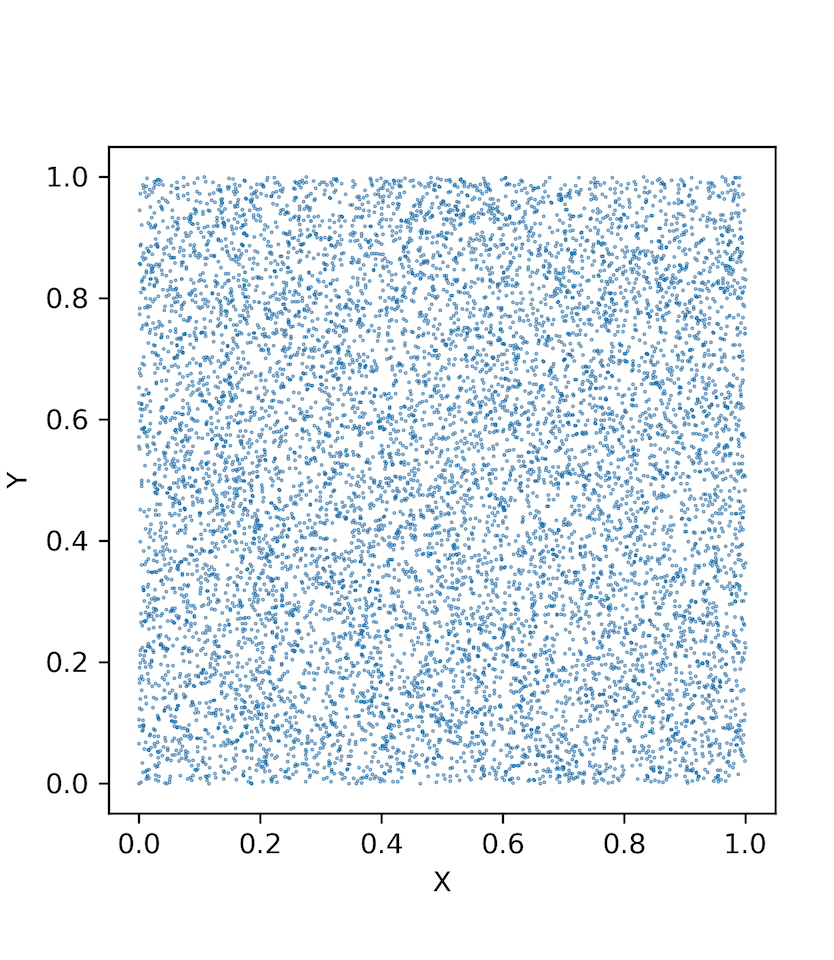
\includegraphics[width=14cm]  {104.png}}        
\caption{\label{1} 由种子“1”生成的$1 \times 10^{4}$个均匀分布随机点}      
\end{figure}

\begin{figure}[!htbp]        
\center{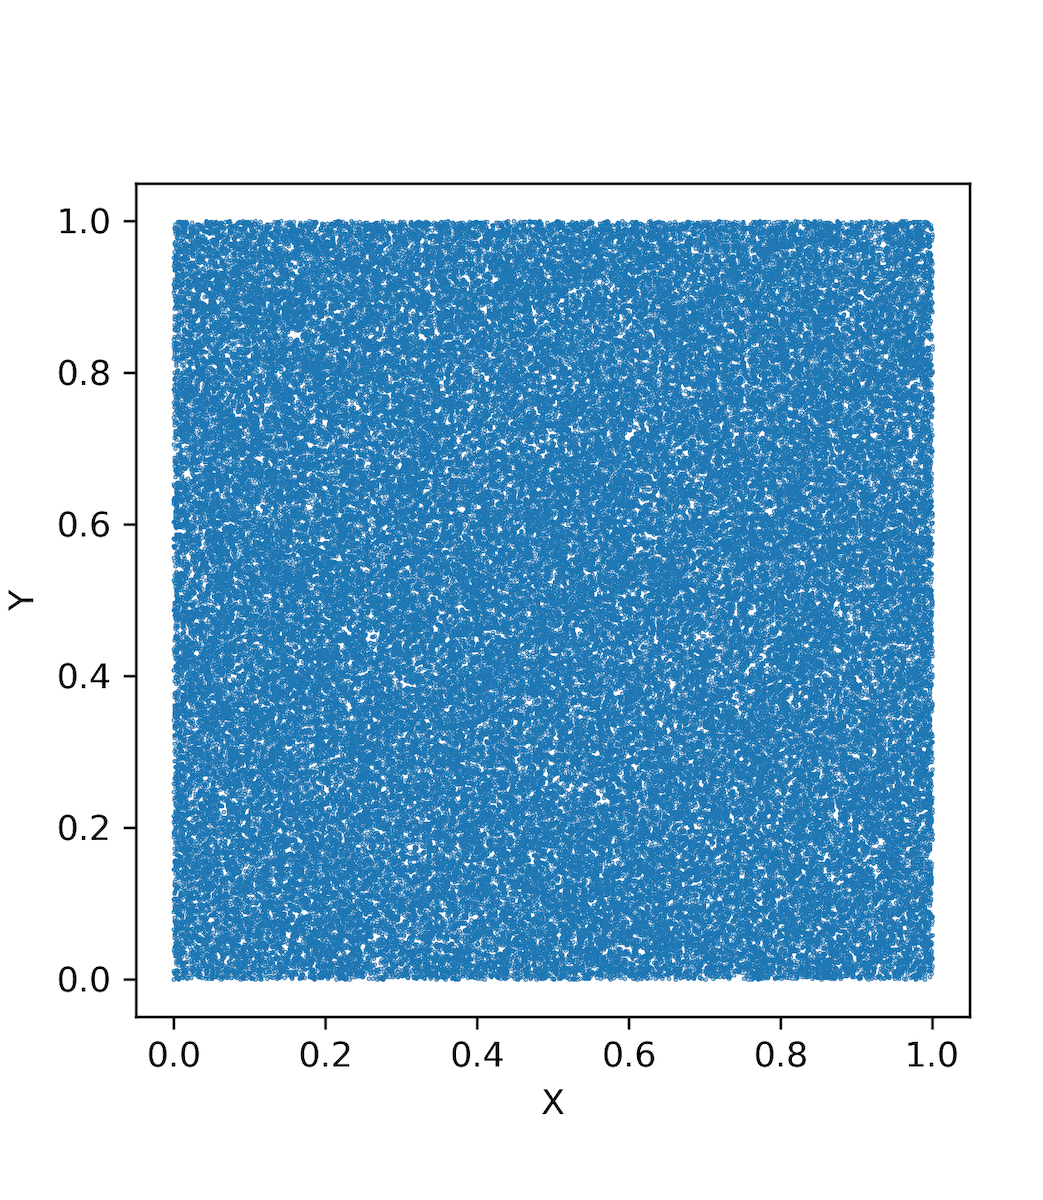
\includegraphics[width=14cm]  {105.png}}        
\caption{\label{1} 由种子“1”生成的$1 \times 10^{5}$个均匀分布随机点}      
\end{figure}

\begin{figure}[!htbp]        
\center{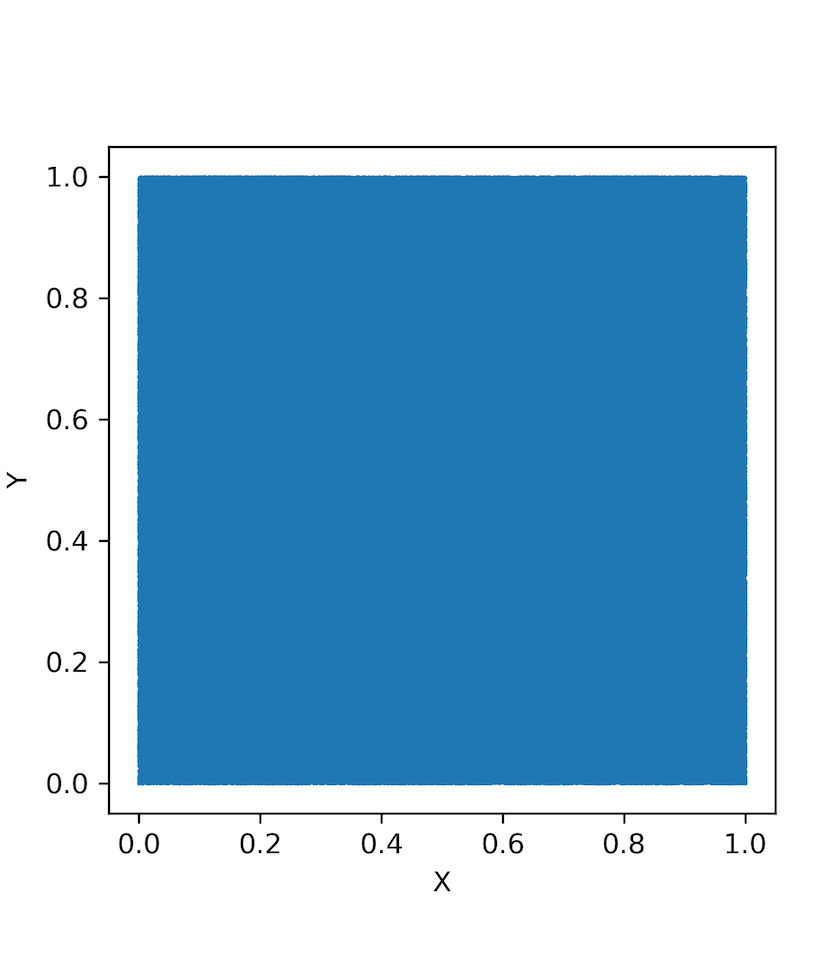
\includegraphics[width=14cm]  {106.png}}        
\caption{\label{1} 由种子“1”生成的$1 \times 10^{6}$个均匀分布随机点}      
\end{figure}

\begin{figure}[!htbp]        
\center{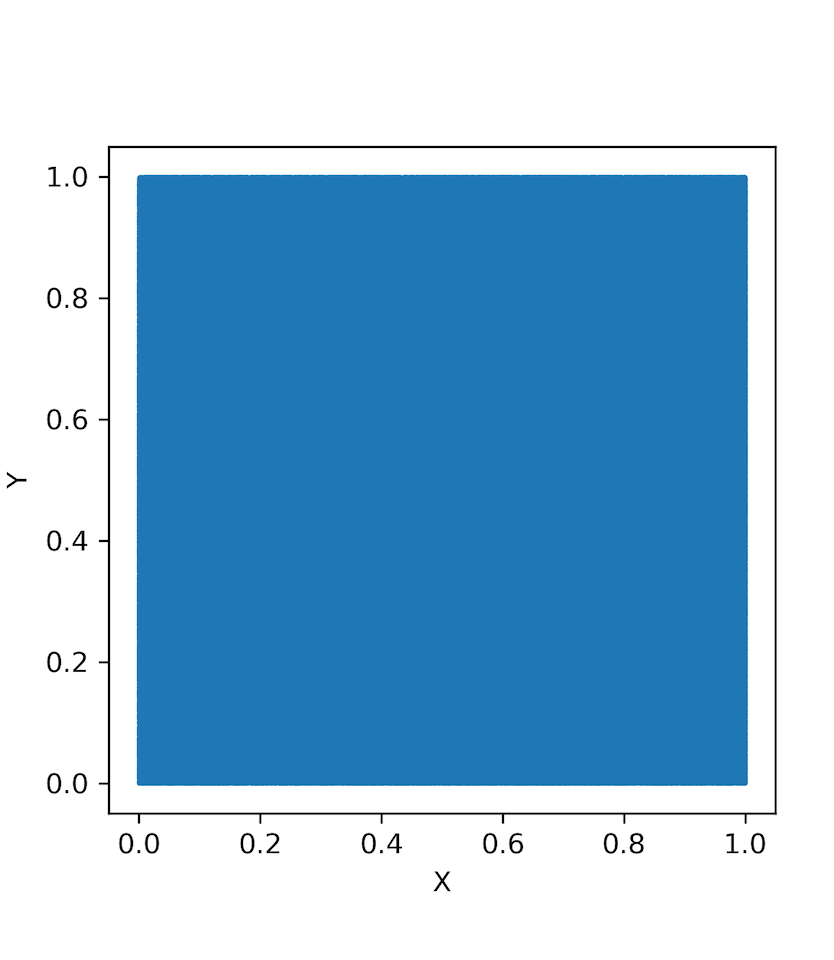
\includegraphics[width=14cm]  {107.png}}        
\caption{\label{1} 由种子“1”生成的$1 \times 10^{7}$个均匀分布随机点}      
\end{figure}

\newpage 从图中我们基本上看不出有条带结构和规则网格结构等有明显规律性的结构\footnote{由于图片分辨率限制,故点数很多时实际上所有$(0,1)$的像素点比总点数要小很多,故此时形成$(0,1)$是一“整块色块”的结果。},可以大致认为随机点见关联性较小。从线性相关系数上看,有下表:
\begin{table}[!htbp]
\centering
\resizebox{\textwidth}{!}{
\begin{tabular}{|c|c|c|c|c|c|c|c|c|c|c|}
\hline
&$N=1 \times 10^{7} $&$N=2 \times 10^{7} $&$N=3 \times 10^{7} $ &$N=4 \times 10^{7} $ &$N=5 \times 10^{7} $  \\ \hline
$C(1)$ &$3.443596 \times 10^{-4}$   & $6.452935\times 10^{-5}$ 
	   & $9.313238\times 10^{-5}$ & $-1.120625 \times 10^{-4}$
	   & $ 7.062223 \times 10^{-5} $  \\ \hline
$C(2)$ &$3.922429\times 10^{-5}$   & $-1.839874\times 10^{-4}$ 
	   & $-1.082820 \times 10^{-4}$ & $-3.138071 \times 10^{-4}$
	   & $ -3.202328 \times 10^{-4} $  \\ \hline
$C(3)$ &$3.617954\times 10^{-4}$   & $2.321942\times 10^{-4}$ 
	   & $1.555808 \times 10^{-4}$ & $2.003216 \times 10^{-4}$
	   & $ 9.992192 \times 10^{-5} $  \\ \hline
$C(4)$ &$-4.454325\times 10^{-5}$   & $2.054347\times 10^{-4}$ 
	   & $3.752631 \times 10^{-5}$ & $3.822061 \times 10^{-5}$
	   & $ 1.845382 \times 10^{-5} $  \\ \hline
$C(5)$ &$-6.123060\times 10^{-5}$   & $5.802567\times 10^{-5}$ 
	   & $6.715514 \times 10^{-5}$ & $6.617884 \times 10^{-5}$
	   & $ 1.476232 \times 10^{-4} $  \\ \hline
$\frac{1}{\sqrt{N}}$ &$3.162278\times 10^{-4}$   & $2.236068\times 10^{-4}$ 
	   & $1.825742 \times 10^{-4}$ & $1.581139 \times 10^{-4}$
	   & $ 1.414214 \times 10^{-4} $  \\ \hline
	   

&$N=6 \times 10^{7} $ &$N=7 \times 10^{7} $ &$N=8 \times 10^{7} $ &$N=9 \times 10^{7} $ &$N=1 \times 10^{8} $ \\ \hline
$C(1)$ & $3.834345 \times 10^{-5}$ & $9.639918 \times 10^{-5}$
	   & $ 6.261886 \times 10^{-5}$ & $4.522615 \times 10^{-5}$
	   & $4.801942 \times 10^{-5}$ \\ \hline
$C(2)$ &$-1.925323\times 10^{-4}$   & $-1.556041\times 10^{-4}$ 
	   & $-1.938455 \times 10^{-4}$ & $-1.909826 \times 10^{-4}$
	   & $ -1.506461 \times 10^{-4} $  \\ \hline
$C(3)$ &$6.037514\times 10^{-5}$   & $6.153215\times 10^{-5}$ 
	   & $3.273687 \times 10^{-5}$ & $7.904676 \times 10^{-5}$
	   & $ 1.029654 \times 10^{-4} $  \\ \hline
$C(4)$ &$3.925839\times 10^{-5}$   & $6.243648\times 10^{-5}$ 
	   & $6.87037 \times 10^{-5}$ & $6.874031 \times 10^{-5}$
	   & $ 7.159278 \times 10^{-5} $  \\ \hline
$C(5)$ &$1.117007\times 10^{-4}$   & $9.083208\times 10^{-5}$ 
	   & $1.036038 \times 10^{-5}$ & $-1.098901 \times 10^{-5}$
	   & $ -3.705724 \times 10^{-5} $  \\ \hline
	   
$\frac{1}{\sqrt{N}}$ &$1.290994\times 10^{-4}$   & $1.195229\times 10^{-4}$ 
	   & $1.118034 \times 10^{-4}$ & $1.054093 \times 10^{-4}$
	   & $ 1.000000 \times 10^{-4} $  \\ \hline

\end{tabular}}
\caption{$C(l)$一览表1}
\end{table}
\newpage 可以看出对于随机数总数$N=i \times 10^{7}$($N=1,3,4,5,6,7,8,9,10$),随机数列的相关系数较大($C(l) $与$ \frac{1}{\sqrt{N}}$量级有时相当),且能看出其线性相关系数随$N$的增大有减小的趋势,不能肯定$x_{n}$和$x_{n+l}$间没有线性关系。而通过比较发现相关系数与$l$之间也没有明显的关系。为了进一步探究$C(l)$是否和$N$,$l$有关,我们又做了如下测试:\footnote{本人仅测试了$l=1,2,3,4,5$,至少这些结论对于这些$l$的取值是成立的}


\begin{table}[!htbp]
\centering
\resizebox{\textwidth}{!}{
\begin{tabular}{|c|c|c|c|c|c|c|c|c|c|c|c|}
\hline
&$N=1 \times 10^{1} $&$N=1 \times 10^{2} $&$N=1 \times 10^{3} $ &$N=1 \times 10^{4} $ &$N=1 \times 10^{5} $&$N=1 \times 10^{6} $  \\ \hline
$C(1)$ &$2.76606\times 10^{-1}$   & $8.989166\times 10^{-2}$ 
	   & $4.054796\times 10^{-2}$ & $-7.021954 \times 10^{-6}$
	   & $ 2.4258476 \times 10^{-3} $ & $ -2.708991 \times 10^{-4} $ \\ \hline
$C(2)$ &$-3.208741\times 10^{-1}$   & $-6.171155\times 10^{-2}$ 
	   & $-2.748282 \times 10^{-2}$ & $-1.144587 \times 10^{-2}$
	   & $ -2.674438 \times 10^{-3} $  & $ -1.717263 \times 10^{-3} $\\ \hline
$C(3)$ &$-1.575569\times 10^{-1}$   & $1.522378\times 10^{-2}$ 
	   & $1.006404 \times 10^{-2}$ & $-5.431764 \times 10^{-3}$
	   & $ 3.505449 \times 10^{-3} $ & $ 8.817028 \times 10^{-4} $ \\ \hline
$C(4)$ &$2.964212\times 10^{-3}$   & $5.501791\times 10^{-2}$ 
	   & $3.450233 \times 10^{-2}$ & $1.437336 \times 10^{-4}$
	   & $ 3.865893 \times 10^{-3} $  & $ -3.776349 \times 10^{-4} $\\ \hline
$C(5)$ &$5.247579\times 10^{-1}$   & $-1.43132\times 10^{-2}$ 
	   & $-7.097997 \times 10^{-3}$ & $-5.586901 \times 10^{-3}$
	   & $ -7.990500 \times 10^{-4} $  & $ -3.313229 \times 10^{-4} $\\ \hline
$\frac{1}{\sqrt{N}}$ &$3.162278\times 10^{-1}$   & $1.000000\times 10^{-1}$ 
	   & $3.162278 \times 10^{-2}$ & $1.000000 \times 10^{-2}$
	   & $ 3.162278 \times 10^{-3} $  & $ 1.000000 \times 10^{-3} $\\ \hline
	   

\end{tabular}}
\caption{$C(l)$一览表2}
\end{table}

由上表可以看出,$C(l)$和$l$确实没有明显的关系,但确实随着$N$的增大而明显的减小。但在不同的$N$的量级下,也总会有$C(l)$比$\frac{1}{\sqrt{N}}$大的情况,所以也不能说16807产生器产生的随机数,其顺序相关较小。


当我们设定$k \in [1,10]$来计算$<x^{k}>$时可得到一下结果:
\begin{table}[!htbp]
\centering
\resizebox{\textwidth}{!}{
\begin{tabular}{|c|c|c|c|c|c|c|c|c|}
\hline
&$N=10^{1}$&$N=10^{2}$&$N=10^{3}$&$N=10^{4}$ &$N=10^{5}$&$N=10^{6}$&$N=10^{7}$&理论值    \\ \hline
 $k=1$(计算值)  & 0.351409 & 0.493705 & 0.491958 & 0.500045 & 0.499777  & 0.500341 & 0.499880 & 0.500000  \\ \hline
 $k=2$(计算值)  & 0.216174 & 0.327029 & 0.323331 & 0.333121 & 0.332932  & 0.333583 & 0.333173 & 0.333333  \\ \hline
 $k=3$(计算值)  & 0.152751 & 0.243376 & 0.239747 & 0.249802 & 0.249505  & 0.250158 & 0.249832 & 0.250000  \\ \hline  
 $k=4$(计算值)  & 0.117402 & 0.193030 & 0.189955 & 0.199907 & 0.199445  & 0.200097 & 0.199835 & 0.200000  \\ \hline
 $k=5$(计算值)  & 0.095795 & 0.159362 & 0.156989 & 0.166714 & 0.166079  & 0.166725 & 0.166507 & 0.166667  \\ \hline  
 $k=6$(计算值)  & 0.081586 & 0.135182 & 0.133601 & 0.143057 & 0.142260  & 0.142893 & 0.142704 & 0.142857  \\ \hline
 $k=7$(计算值)  & 0.071592 & 0.116897 & 0.116170 & 0.125347 & 0.124409  & 0.125022 & 0.124853 & 0.125000  \\ \hline 
 $k=8$(计算值)  & 0.064114 & 0.102531 & 0.102685 & 0.111595 & 0.110536  & 0.111125 & 0.110970 & 0.111111  \\ \hline
 $k=9$(计算值)  & 0.058209 & 0.090916 & 0.091945 & 0.100606 & 0.099447  & 0.100010 & 0.099865 & 0.100000  \\ \hline
 $k=10$(计算值) & 0.053334 & 0.081314 & 0.083188 & 0.091620 & 0.090382  & 0.090917 & 0.090779 & 0.090909  \\ \hline

\end{tabular}}
\caption{$<x^{k}>$ 一览表}
\end{table}
 
 
\begin{table}[!htbp]
\centering
\resizebox{\textwidth}{!}{
\begin{tabular}{|c|c|c|c|c|c|c|c|}
\hline
&$N=10^{1}$&$N=10^{2}$&$N=10^{3}$&$N=10^{4}$ &$N=10^{5}$&$N=10^{6}$&$N=10^{7}$    \\ \hline
 $k=1$(计算值)  & 0.148591 & 0.006295 & 0.008042 & 0.000045 & 0.000223  & 0.000341 & 0.000120  \\ \hline
 $k=2$(计算值)  & 0.117159 & 0.006304 & 0.010002 & 0.000212 & 0.000401  & 0.000249 & 0.000161  \\ \hline
 $k=3$(计算值)  & 0.097249 & 0.006624 & 0.010253 & 0.000198 & 0.000495  & 0.000158 & 0.000168   \\ \hline  
 $k=4$(计算值)  & 0.082598 & 0.006970 & 0.010045 & 0.000093 & 0.000555  & 0.000097 & 0.000165  \\ \hline
 $k=5$(计算值)  & 0.070872 & 0.007304 & 0.009677 & 0.000048 & 0.000587  & 0.000059 & 0.000160   \\ \hline  
 $k=6$(计算值)  & 0.061271 & 0.007675 & 0.009256 & 0.000199 & 0.000597  & 0.000036 & 0.000153  \\ \hline
 $k=7$(计算值)  & 0.053408 & 0.008103 & 0.008830 & 0.000347 & 0.000591  & 0.000022 & 0.000147  \\ \hline 
 $k=8$(计算值)  & 0.046997 & 0.008580 & 0.008426 & 0.000484 & 0.000575  & 0.000014 & 0.000141  \\ \hline
 $k=9$(计算值)  & 0.041791 & 0.009084 & 0.008055 & 0.000606 & 0.000553  & 0.000010 & 0.000135  \\ \hline
 $k=10$(计算值) & 0.037575 & 0.009595 & 0.007721 & 0.000711 & 0.000527  & 0.000008 & 0.000130  \\ \hline
 $\frac{1}{\sqrt{N}}$    & 0.316228 & 0.10000 & 0.031623 & 0.010000 & 0.003162  & 0.001000 & 0.000316  \\ \hline

\end{tabular}}
\caption{$<x^{k}>$与理论值差别的绝对值一览表}
\end{table}
 
 \newpage 由上表看出,当$N$越大时,随机点的$<x^{k}>$越接近于理想均匀分布的理论值。在$N\leq 10^{7}$时与理论值的差别控制在$\frac{1}{\sqrt{N}}$以内,可认为此方法产生的随机点分布较为均匀。



\section{心得与体会}
通过此次作业结果,发现比较简单的16807随机数产生器比预想的要好一点,之前以为画出的随机点的图像上会有明显的规律性结构,在此问题下此随机数产生器还是有可用性的。但是其顺序相关性还是不能够认为是比较小的,故在某些需要顺序相关性比较小的情况下,还是不能够使用此产生器产生随机数。

另外也是第一次编程作业的缘故,也有大致复习了(重学)了一遍C语言的作用。另外也发现要给数组开辟较大的空间时,要采用malloc()函数,从堆上开辟空间,直接按静态数组定义,会造成栈空间的不够从而报错(全局数组例外)的trick。还有就是也熟悉了一下\LaTeX 。
\newpage
\section{附录}

\begin{appendices}
\section{C语言程序源码}

\begin{lstlisting}[language = C]
#include <stdio.h>
#include <stdlib.h>
#include <time.h>
#include <math.h>
#define a 16807
#define b 0
#define m 2147483647
#define r (m % a)
#define q (m / a)


//写文件子程序,输入写成文件名称字符串str,数据来源于数组num,数据总数n
int my_filewriter(char str[],double num[],int n){
    FILE * fp;
    fp = fopen(str,"w+");

    for(int i=0;i<(n-1);i++)
    {
        fprintf(fp,"%lf,",num[i]);

    }
    fprintf(fp,"%lf",num[n]);    //最后一个数据后不加 ","
    fclose(fp);
    return 0;
}



// Schrage 方法产生随机数
int my_schrage(double ran[],int ranI[],int n){
    for (int i = 0; i < n - 1; i++) {
        if (ranI[i] >= 0) {
            ran[i] = ranI[i] / (double) m;
        } else {
            ran[i] = (ranI[i] + m) / (double) m;
        }
        if(ranI[i] == m-1){
            if(a >=  b){    //由于Schrage方法只对z in (0,m-1)成立,故这里要讨论z == m-1的情况
                ranI[i+1] = m + (b-a) % m;
            }
            else   ranI[i+1] =  (b-a) % m;

        }
        else ranI[i+1] = ((a * (ranI[i] % q) - r *( ranI[i] /  q) ) + b % m ) % m;  //递推式
    }
    if (ranI[n-1] >= 0) {
        ran[n-1] = ranI[n-1] / (double) m;
    } else {
        ran[n-1] = (ranI[n-1] + m) / (double) m;
    }
    return 0;
}





//线性相关检验
int my_cl_check(double ranx[],double rany[],int n){
    long double xy = 0;  //sum(x*y)
    long double x = 0;   //sum(x)
    long double x2 = 0;  //sum(x^2)
    double cl = 0;
    for(int i = 0;i<n;i++){
        xy += ranx[i] * rany[i];
        x += ranx[i];
        x2 += pow(ranx[i],2);
    }
    cl = ((xy/n)-pow(x/n,2))/(pow(x,2)/n -pow(x/n,2));   //C(l)计算
    printf("所产生的%d 个随机点的线性相关系数 C(l) = %E\n",n,cl);
    return 0;
}



//<x^k>测试均匀性
int my_xk_check(double ranx[],double rany[],int n,int k){
    double sumxk[k];    //sum(x^k)
    double sumyk[k];    //sum(y^k)
    for(int j = 0;j < k;j++){    //初始化数组
        sumxk[j] = 0;
        sumyk[j] = 0;
    }

    for(int i = 0;i < n;i++){     //数组赋值
        for(int j = 0;j < k;j++){
            sumxk[j] += pow(ranx[i],j+1);
            sumyk[j] += pow(rany[i],j+1);
        }
    }
    for(int j = 0;j < k;j++){    //计算<x^k>,<y^k>
        sumxk[j] = sumxk[j]/n;
        printf("N = %-8d <x^%d> = %lf  with theoretical number of %lf\n",n,j+1,sumxk[j],1.0/(2+j));
        sumyk[j] = sumyk[j]/n;
        //printf("N = %-8d <y^%d> = %lf  with theoretical number of %lf\n",n,j+1,sumyk[j],1.0/(2+j));
        //此子程序还可用来计算<y^k>
    }


    return 0;
}



int main() {
    int N; //总随机数个数,即x坐标随机数值+y坐标随机数值(即必须为偶数)
    char str[50];
    printf("请输入您所需要的总点数:");
    while (!scanf("%d",&N)) {  //简单的输入检查
        gets(str);
        printf("\nInput error,please try again\n");
        printf("请输入您所需要的总点数:");
    }
    N=2*N;
    if(N >2000000) printf("您输入的参数已接受,正在计算请稍等片刻~\n");

    double *ran = malloc(sizeof(double) * N);  //用来存放随机数
    int *ranI = malloc(sizeof(int) * N);    //用来存放递推数列
    ranI[0]=1;   //产生一个种子值放入ranI的第一项

    my_schrage(ran,ranI,N);
    
    double *ranx = malloc(sizeof(double) * N/2);
    double *rany = malloc(sizeof(double) * N/2);

    for(int i=0;i<N;i=i+2){     //将ran[]中相邻的两个随机数分别赋值到ranx[]和rany[]
        ranx[i/2]=ran[i];
        rany[i/2]=ran[i+1];
    }
    my_filewriter("ranx.dat",ranx,N/2);
    my_filewriter("rany.dat",rany,N/2);
    my_cl_check(ranx,rany,N/2);

    int k;
    printf("Please input the max value of k in <x^k>:");
    while (!scanf("%d",&k)) {  //简单的输入检查
        gets(str);
        printf("\nInput error,please try again\n");
        printf("Please input the max value of k in <x^k>:");
    }
    printf("以下是<x^k>的均匀性测试:\n");
    for(int j = N/10 ;j >= 1 ;j = j/10){    //进行<x^k>均匀性测试
        my_xk_check(ranx,rany,N/j,k);
    }

    return 0;
}
\end{lstlisting}

\newpage
\section{可视化python脚本源程序}
\begin{lstlisting}[language = python]
import matplotlib.pyplot as plt
import numpy as np
from IPython.core.pylabtools import figsize # import figsize
#figsize(12.5, 4) # 设置 figsize
plt.rcParams['savefig.dpi'] = 300 #图片像素
plt.rcParams['figure.dpi'] = 300 #分辨率

fig = plt.figure()
ax = fig.add_axes([0.1, 0.1, 0.8, 0.8])
X = []
Y = []

with open('cmake-build-debug/ranx.dat', 'r') as f:  #依数据文件所在位置而变
    while True:
        lines = f.readline() # 整行读取数据
        if not lines:
            break
            pass
        tmp = [float(i) for i in lines.split(',')] # 将整行数据分割处理        
        X.append(tmp)  # 添加新读取的数据
        pass
    X = np.array(X) # 将数据从list类型转换为array类型。
pass

    
with open('cmake-build-debug/rany.dat', 'r') as f:  #依数据文件所在位置而变

    while True:
        lines = f.readline() # 整行读取数据
        if not lines:
            break
            pass
        tmp = [float(i) for i in lines.split(',')] # 将整行数据分割处理        
        Y.append(tmp)  # 添加新读取的数据
        pass
    Y = np.array(Y) # 将数据从list类型转换为array类型。
pass
    
    
    
# 绘制散点图
ax.scatter(X, Y, s=0.1)    #画散点图
ax.set_aspect('equal')
ax.set_xlabel('X')
ax.set_ylabel('Y')
plt.savefig("random(x,y).png")

\end{lstlisting}

\end{appendices}







\end{document}
